\section{理论}
\subsection{经典PageRank}
Google的PageRank算法是特征向量中心性的变型。PageRank向量 由下式给出

\begin{equation}
	GI_{c1}=I_{c1}
\end{equation}

G是Google矩阵,定义为如下

\begin{equation}
	G:=\alpha E+\frac{1-\alpha}{N}1
\end{equation}

这里$N$是网络阶结点数量,$E$是一个邻接矩阵,$\alpha$是衰减参数(一般$\alpha$为0.85),$1$是一个全为1的矩阵。一般来说,第二项代表步行器跳到网络其他节点的概率。

定义网络邻接矩阵$C$,当结点$k$和$j$有边时$C_{jk}=1$,否则$C_{jk}=0$。为了得到$E$,$C$需要被修改以便每个包含所有0的列$k$(对应于0个出度的节点k1)被一个所有项都设置为$\frac{1}{N}$的列替换。剩下的有出度的列通过除以结点出度正规化到总和为1。将一个节点$k$出度表示为$D_k$,使得$D_k=\sum_{j}C_{jk}$。用数学来表示如下

\begin{equation}
	E_{jk}=\begin{cases}
	\frac{1}{N} & {\rm if}\ D_k=0\\
	\frac{C_{jk}}{D_k} & {\rm if}\ D_k\neq 0
	\end{cases}
\end{equation}

\subsection{离散时间量子行走的Szegedy-Google PageRank}

Szegedy的离散时间的形式是对应于经典随机行走的马尔科夫链的量子化。传统上,对于$N$节点图,这样的过程由转移概率的$N$×$N$矩阵$P$描述,其中$P_jk$表示从节点$k$到节点$j$的转移概率。Szegedy行走在希尔伯特空间$\mathcal { H } ^ { N ^ { 2 } } = \mathcal { H } ^ { N } \otimes \mathcal { H } ^ { N }$发生。这个空间是所有向量$| j , k \rangle$的范围,其中每个向量表示从节点$j$到节点$k$的图中的有向边。

首先,我们定义状态向量如下

\begin{equation}
	\begin{aligned} | \psi _ { j } \rangle & : = | j \rangle \otimes \sum _ { k = 1 } ^ { N } \sqrt { P _ { k j } } | k \rangle \\ & = \sum _ { k = 1 } ^ { N } \sqrt { P _ { k j } } | j , k \rangle \end{aligned}
\end{equation}

对于图的每一个节点$j = 1 , \dots , N$,这表示边状态$| j \rangle _ { 1 } | k \rangle _ { 2 }$的叠加来自第$j$个节点,被$P$赋予权重。投影算子如下

\begin{equation}
	\hat { \Pi } : = \sum _ { j = 1 } ^ { N } | \psi _ { j } \rangle \left\langle \psi _ { j } |\right.
\end{equation}
和
\begin{equation}
	\hat { S } : = \sum _ { j , k = 1 } ^ { N } | j , k \rangle \langle k , j |
\end{equation}

是交换算子。量子行走的步长为统一的算子

\begin{equation}
	\hat { U } : = \hat { S } ( 2 \hat { \Pi } - \hat { \mathbbm { 1 } } )
\end{equation}

然而二步演算算子的形式为

\begin{equation}
	\hat { U } ^ { 2 } : = ( 2 \hat { S } \hat { \Pi } \hat { S } - \hat { \mathbbm { 1 } } ) ( 2 \hat { \Pi } - \hat { \mathbbm { 1 } } )
\end{equation}

正如[4]中提出的,使用Google矩阵$G$作为随机矩阵$P$实现了经典PageRank算法的量子版本。 由于$G$是随机的,因此保持量子行走的单一性; 此外,$G$中保留了有关网络方向性的信息。

相应的量子走路初始化为

\begin{equation}
	| \psi _ { 0 } \rangle = \frac { 1 } { \sqrt { N } } \sum _ { j = 1 } ^ { N } | \psi _ { j } \rangle
\end{equation}

也就是说所有节点之间的相等叠加,但在每个节点的边缘状态之间由$G$加权。以$\hat{U}^2$作为步行的离散时间演化算子,瞬时量子PageRank则是

\begin{equation}
	I _ { q } \left( P _ { i } , t \right) = \left\langle \psi _ { 0 } \left| \hat { U } ^ { \dagger 2 t } \right| i \right\rangle _ { 2 } \left\langle i \left| \hat { U } ^ { 2 t } \right| \psi _ { 0 } \right\rangle
\end{equation}

它被定义为在$t$个时间步之后步行器在网络中$P_i$页面的概率分布。 由于由方程式定义的量子行走算子的统一性和可逆性,该值不会及时收敛到任何静态分布。

因为一个量子PageRank度量必须为每个节点提供一个特殊的排序,Paparo等人将它定义为步行器时间平均概率分布:

\begin{equation}
	I _ { \mathrm { TA } } \left( P _ { i } \right) : = \left\langle I _ { q } \left( P _ { i } , t \right) \right\rangle = \frac { 1 } { t _ { \mathrm { max } } } \sum _ { t = 0 } ^ { t _ { \max } - 1 } I _ { q } \left( P _ { i } , t \right)
\end{equation}

它会在足够大的$t_{max}$时收敛。这在这篇文章中被称为时间平均PageRank度量。

我们根据在节点上找到步行器的峰值概率提出了另一种PageRank度量。我们使用在$t_{max}$之后达到的最大$I_q(P_i,t)$作为节点的量子PageRank:

\begin{equation}
	I _ { P _ { \max } } \left( P _ { i } \right) : = \max \left\{ I _ { q } \left( P _ { i } , t \right) : 1 \leq t \leq t _ { \max } , t \in \mathbbm { Z } \right\}
\end{equation}

我们想基于公式(10)中的$I_q(P_i,t)$的振荡演化来测量一个合适的时间量程$t_{max}$。首先,我们使用$t$=500倍的$\hat{U}^2$步长作为初始状态。对时间序列$I_q(P_i,t)$执行傅立叶变换产生其中存在的振荡频率的功率谱。我们定义为$\omega \left( P _ { i } \right)$噪声之上的最低频率,该噪声使用最高峰值的10%来作为阈值。$I_q(P_i,t)$的周期是$T _ { q } \left( P _ { i } \right) = \frac { 2 \pi } { \omega \left( P _ { i } \right) }$。一般来说,网络中与页面$P_i$关联的每个节点$i$都有一个不同的周期$T_q(P_i)$。

使用$\left\langle T _ { q } ^ { a l l } \right\rangle$来表示所有节点的平均周期。

\begin{equation}
	\left\langle T _ { q } ^ { a l l } \right\rangle : = \frac { 1 } { N } \sum _ { i = 1 } ^ { N } T _ { q } \left( P _ { i } \right)
\end{equation}

\begin{figure}[h]
	\centering
	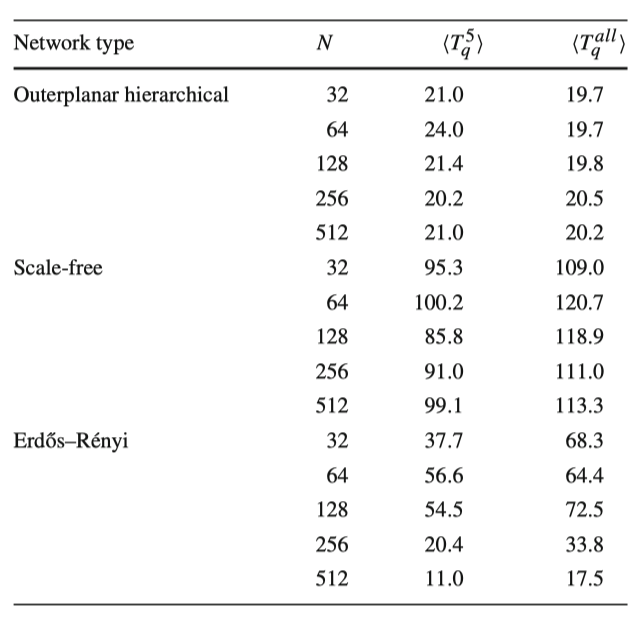
\includegraphics{part/pic/table1.png}
	\caption{\ 对于$N$个节点,平均周期$\left\langle T _ { q } ^ { 5 } \right\rangle$和三个网络类型的$\left\langle T _ { q } ^ { a l l } \right\rangle$}
\end{figure}

令$\left\langle T _ { q } ^ { 5 } \right\rangle$为瞬时量子PageRank节点的平均周期,其瞬时量子PageRanks的$I _ { q } \left( P _ { j } , t \right)$在各自周期$1 \leq t \leq T _ { q } \left( P _ { j } \right) , t \in \mathbbm { Z }$内达到最高峰值。

按照上述步骤,我们计算与本研究相关的定向网络系列的$\left\langle T _ { q } ^ { a l l } \right\rangle$和$\left\langle T _ { q } ^ { 5 } \right\rangle$,即外平面分层、无标度和ER网络,大小为$N$ = 32,54,128,256,512个节点。我们使用对于每个$N$十个无标度和ER随机网络的集合,这些网络由NetworkX [13]生成。对于此处和本文中的每个ER网络,边连接的概率设置为$p$ = 0.07。 我们使用$t_max = 2 \left\langle T _ { q } ^ { 5 } \right\rangle$作为我们的PageRank分析所需的时间尺度,推断在确定每个网络的一般时间尺度时,大多数中心节点的周期应该比周边节点的周期更强。

数值结果如图1所示,图2绘制了平均周期与网络规模的比例。我们的结果表明,$t_{max} = 2 \left\langle T _ { q } ^ { 5 } \right\rangle$不会随$N$线性向上扩展,而是对于此处考虑的网络类型保持稳定。在确定性构建的外平面分层网络的情况下,对于连续过程中,在大约$\langle T \rangle = 20$时间步长的平均周期平稳。总体而言,无标度网络的平均周期最高。我们看到较大的ER网络(具有相同的边缘概率$p$ = 0.07)倾向于具有较小的平均周期。我们预计较高$N$的时间尺度将保持有限。

这是一个重要的发现,因为它提供了有效实施量子PageRank方案的可能性,这是文献中尚未解决的关键问题。请注意Chiang等人[14]提出了一个有效的量子电路来实现Szegedy在任意稀疏网络上的行走。 尽管在$I_{TA}$和$I_{OS}$中使用Google矩阵会导致相关的统一演化算子$\hat{U}$变得密集,但Loke和Wang[15]利用将Google矩阵划分为可管理的子集并扩展了Chiang等人的方案。只要原始网络稀疏,就可以有效地实现Google矩阵。

\begin{figure}[h]
	\centering
	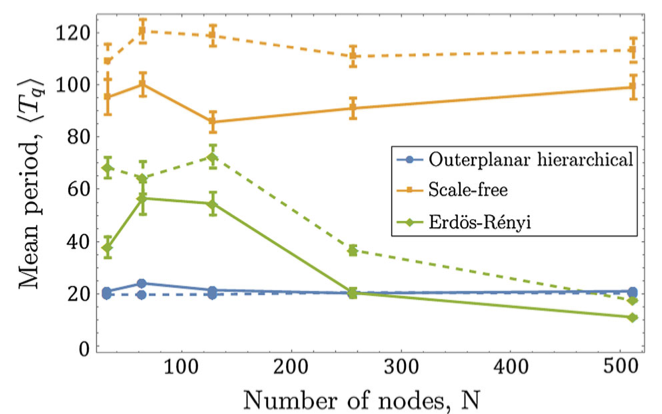
\includegraphics{part/pic/fig1.png}
	\caption{$N$ = 32,64,128,256,512个节点的网络大小的平均周期缩放。 外平面分层,无标度和ER网络的平均周期$\left\langle T _ { q } ^ { 5 } \right\rangle$(实线)和$\left\langle T _ { q } ^ { all } \right\rangle$(虚线)分别绘制为蓝色,橙色和绿色。对于无标度和ER随机网络,每个N使用十个图的集合。每个误差条对应于来自每个集合的十个$\left\langle T _ { q } \right\rangle$值的平均值的标准误差}
\end{figure}

\subsection{通过连续时间量子遍历开放系统PageRank}

连续时间量子步行最初是由Farhi和Gutmann[16]提出的,它是根据决策树重新计算的计算问题的研究。遵循薛定谔方程,这种演化被描述为

\begin{equation}
	\frac { \mathrm { d } | \Psi ( t ) \rangle } { \mathrm { d } t } = - i \hat { H } | \Psi ( t ) \rangle
\end{equation}

其中$\hat{H}$是转换率矩阵。在量子力学中需要单一演化算子意味着$\hat{H}$必须是Hermitian,通常不是定向行走的情况。为了向CTQW引入方向性,我们采用Lindblad-von Neumann方程的开放系统方法,该方程解释了通过与外部环境配合的有向步行的非单一性质。

为了使用开放量子系统,密度算子的概念被用来替代量子力学中波函数。系统的密度算子由[17]定义

\begin{equation}
	\rho = \sum _ { i = 1 } ^ { N } p _ { i } | \Psi _ { i } \rangle \left\langle \Psi _ { i } |\right.
\end{equation}

其中$p_i$是表示状态多少的常量,$| \Psi _ { i } \rangle$是最终混合状态,其中$\sum _ { i = 1 } ^ { N } p _ { i } = 1$。

Lindblad-von Neumann方程描述了量子系统在追踪环境后如何演变,并且可以以[18]的形式编写:

\begin{equation}
	\frac { \mathrm { d } \rho } { \mathrm { d } t } = - i \hbar [ \hat { H } , \rho ] + \sum _ { k } \gamma _ { k } \left( \hat { L } _ { k } \rho \hat { L } _ { k } ^ { \dagger } - \frac { 1 } { 2 } \left\{ \hat { L } _ { k } \hat { L } _ { k } ^ { \dagger } , \rho \right\} \right)
\end{equation}

其中$\hat{L}_k$是$\rho$所在空间上的单一算子。所有$\hat{L}_k$的集合构成了这个空间的基础。矩阵$\gamma$描述了诸如温度之类的非节能现象如何影响系统。

在经典(无向)和经典(有向)行为之间的顶部参数插值,衰减参数$\beta$被引入到Lindblad-von Neumann方程:

\begin{equation}
	\frac { \mathrm { d } \rho } { \mathrm { d } t } = - i ( 1 - \beta ) [ \hat { H } , \rho ] + \beta \sum _ { i , j } \gamma _ { i j } \left( \hat { L } _ { i j } \rho \hat { L } _ { i j } ^ { \dagger } - \frac { 1 } { 2 } \left\{ \hat { L } _ { i j } \hat { L } _ { i j } ^ { \dagger } , \rho \right\} \right)
\end{equation}

其中$\hat{H}$是邻接矩阵$C$的对称形式,表示其对应的无向图。 根据方程(3),将$\gamma$作为邻接矩阵$E$。 这是当$\alpha=1$时公式(2)中Google矩阵G的特定情况。我们的方法等同于Sánchez-Burillo等人开发的量子PageRank算法,他们设置$\gamma = G$且$\alpha= 0.9$。

我们通过Saalfrank使用的本征算子方法求解主方程。这是一种线性化方法,将非线性方程转化为线性方程,由此使方程(17)变成

\begin{equation}
	\frac { \mathrm { d } \rho } { \mathrm { d } t } = - i ( 1 - \beta ) \mathcal { L } _ { H } \rho + \beta \mathcal { L } _ { D } \rho = \mathcal { L } _ { S O } \rho
\end{equation}

这使得从原始$N$维空间的本征操作符$\mathcal { L } _ { H }$和$\mathcal { L } _ { D }$到$N^2$维的空间,并且在该设置中对密度矩阵进行矢量化。

根据公式(18),$\mathcal { L } _ { H }$和$\mathcal { L } _ { D }$可以组合成一个算子$\mathcal { L } _ { SO }$。对于与时间无关的$\mathcal { L } _ { SO }$,通过取$\mathcal { L } _ { SO }$的矩阵指数,在任何时间$t$都可以很容易地求解这种形式,即

\begin{equation}
	\rho = \rho _ { 0 } e ^ { \mathcal { L } _ { S O t } }
\end{equation}

保证了对于足够大的$t$的稳定结果的收敛,每个节点的占用概率表示开放系统量子PageRank,即

\begin{equation}
	I _ { \mathrm { OS } } \left( P _ { i } \right) : = \langle i | \rho | i \rangle = \rho _ { i i }
\end{equation}